% ------------------------------------------------------------------------------
% TYPO3 CMS 8.6 - What's New - Chapter "Introduction" (Spanish Version)
%
% @author	Michael Schams <schams.net>
% @license	Creative Commons BY-NC-SA 3.0
% @link		http://typo3.org/download/release-notes/whats-new/
% @language	English
% ------------------------------------------------------------------------------
% LTXE-CHAPTER-UID:		7fdf26cc-362160ab-d6c8b905-19722b20
% LTXE-CHAPTER-NAME:	Introduction
% ------------------------------------------------------------------------------

\section{Introduction}
\begin{frame}[fragile]
	\frametitle{Introducción}

	\begin{center}\huge{Introducción}\end{center}
	\begin{center}\huge{\color{typo3darkgrey}\textbf{Los Hechos}}\end{center}

\end{frame}

% ------------------------------------------------------------------------------
% LTXE-SLIDE-START
% LTXE-SLIDE-UID:		6e296c20-18119972-25da7ae2-89451cb2
% LTXE-SLIDE-ORIGIN:	ea30ee1a-0bc39e0a-bcaf8d4b-fccc3d18 English
% LTXE-SLIDE-TITLE:		TYPO3 CMS 8.6 - The Facts
% ------------------------------------------------------------------------------
\begin{frame}[fragile]
	\frametitle{Introducción}
	\framesubtitle{TYPO3 CMS 8.6 - Los Hechos}

	\begin{itemize}
		\item Fecha de lanzamiento: 14 February 2017
		\item Tipo de lanzamiento: Lanzamiento Sprint
		\item Eslogan: "Puliendo"
	\end{itemize}

	\begin{figure}
		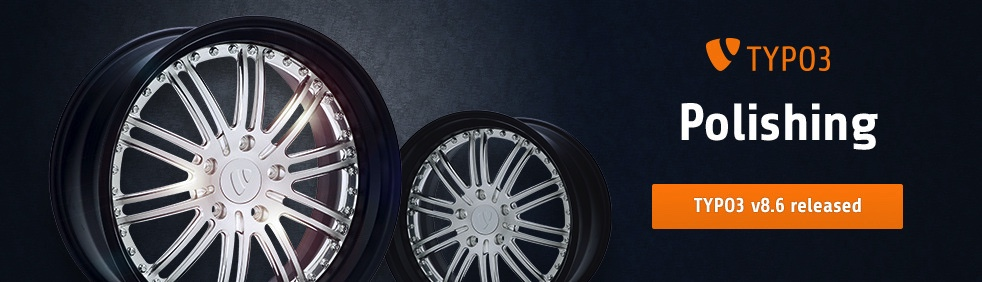
\includegraphics[width=0.95\linewidth]{Introduction/typo3cms86-banner.jpg}
	\end{figure}

\end{frame}

% ------------------------------------------------------------------------------
% LTXE-SLIDE-START
% LTXE-SLIDE-UID:		bfe66e41-be580061-6f6e0476-f06bf078
% LTXE-SLIDE-ORIGIN:	edf38742-589c1a34-ae855361-e0284741 English
% LTXE-SLIDE-TITLE:		System Requirements
% ------------------------------------------------------------------------------
\begin{frame}[fragile]
	\frametitle{Introducción}
	\framesubtitle{System Requirements}

	\begin{itemize}
		\item PHP:\tabto{2.2cm}versión 7
		\item MySQL:\tabto{2.2cm}versión 5.5 a 5.7
		\item Espacio de disco:\tabto{2.2cm}mín 200 MB
		\item Ajustes PHP:

			\begin{itemize}
				\item \texttt{memory\_limit} >= 128M
				\item \texttt{max\_execution\_time} >= 240s
				\item \texttt{max\_input\_vars} >= 1500
				\item opción de compilación \texttt{-}\texttt{-disable-ipv6} \underline{no} debe usarse
			\end{itemize}

		\item El backend requiere Microsoft Internet Explorer 11 o posterior,
			Microsoft Edge, Google Chrome, Firefox, Safari o cualquier otro navegador
			moderno y compatible

	\end{itemize}

\end{frame}

% ------------------------------------------------------------------------------
% LTXE-SLIDE-START
% LTXE-SLIDE-UID:		7ff14bf5-d9ad5726-b5dab77d-d19135bf
% LTXE-SLIDE-ORIGIN:	8cb2705f-d045b3fa-b2ca4f81-52d16aef English
% LTXE-SLIDE-TITLE:		Development And Release Timeline
% ------------------------------------------------------------------------------
\begin{frame}[fragile]
	\frametitle{Introducción}
	\framesubtitle{Línea de tiempo de Desarrollo y Lanzamiento}

	\begin{figure}
		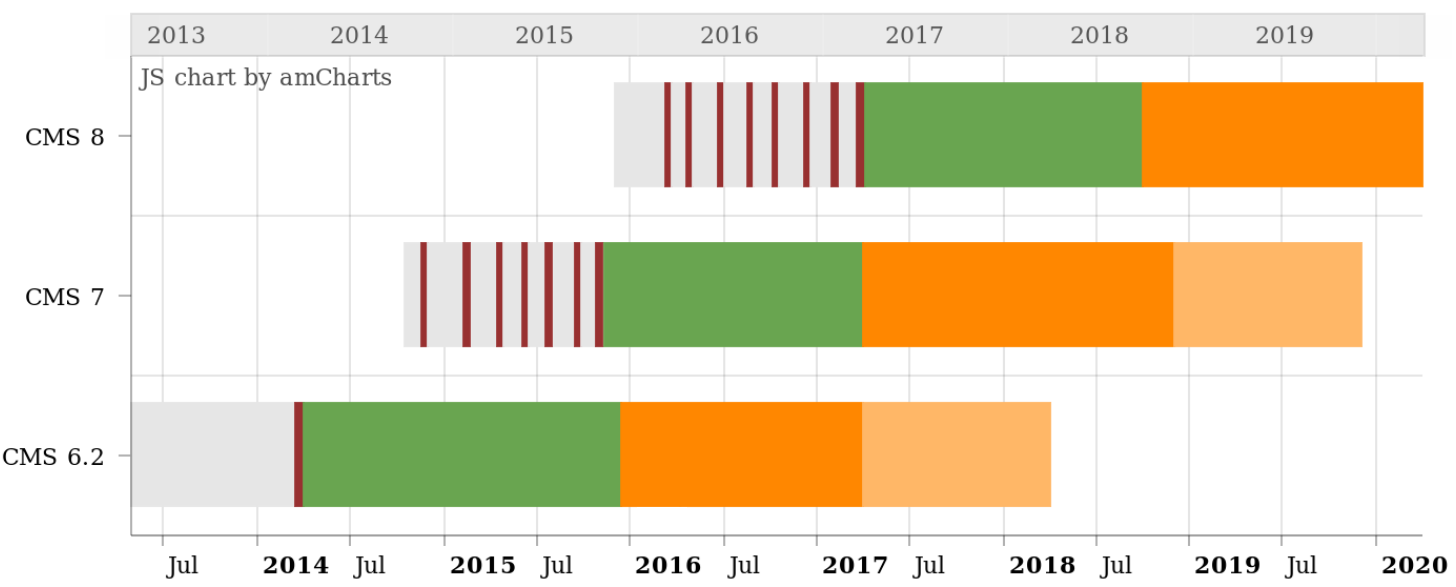
\includegraphics[width=1\linewidth]{Introduction/ReleaseAgenda.png}
	\end{figure}

\end{frame}

% ------------------------------------------------------------------------------
% LTXE-SLIDE-START
% LTXE-SLIDE-UID:		1c43a90b-7c2f9423-8da8dc36-11aaef2e
% LTXE-SLIDE-ORIGIN:	dae3f732-e4550c37-dc304056-f090affc English
% LTXE-SLIDE-TITLE:		TYPO3 CMS Roadmap
% ------------------------------------------------------------------------------
\begin{frame}[fragile]
	\frametitle{Introducción}
	\framesubtitle{Línea de lanzamiento de TYPO3 CMS}

	Fechas de lanzamiento y sus enfoques principales:

	\begin{itemize}

		\item v8.0 \tabto{1.1cm}22/Mar/2016\tabto{3.4cm}Añadiendo cosas de última hora
		\item v8.1 \tabto{1.1cm}03/May/2016\tabto{3.4cm}Integración con la Nube
		\item v8.2 \tabto{1.1cm}05/Jul/2016\tabto{3.4cm}Requisitos previos Doctrine
		\item v8.3 \tabto{1.1cm}30/Ago/2016\tabto{3.4cm}Editor de Texto Enriquecido
		\item v8.4 \tabto{1.1cm}18/Oct/2016\tabto{3.4cm}Migración a Doctrine + Actualizaciones
		\item v8.5 \tabto{1.1cm}20/Dic/2016\tabto{3.4cm}Nuevo RTE + Soporte de Integrador
		\item
			\begingroup
				\color{typo3orange}
					v8.6 \tabto{1.1cm}14/Feb/2017\tabto{3.4cm}Puliendo
			\endgroup
		\item v8.7 \tabto{1.1cm}04/Abr/2017\tabto{3.4cm}Preparación LTS

	\end{itemize}

	\smaller
		\url{https://typo3.org/typo3-cms/roadmap/}\newline
		\url{https://typo3.org/news/article/kicking-off-typo3-v8-development/}
	\normalsize

\end{frame}

% ------------------------------------------------------------------------------
% LTXE-SLIDE-START
% LTXE-SLIDE-UID:		2ebab17d-1b8b1715-61ed192e-d8cb685d
% LTXE-SLIDE-ORIGIN:	4a382358-6fd84263-041bc029-bd50bb1e English
% LTXE-SLIDE-TITLE:		Installation
% ------------------------------------------------------------------------------
\begin{frame}[fragile]
	\frametitle{Introducción}
	\framesubtitle{Installation}

	\begin{itemize}
		\item Procedimiento de instalación \textit{clásico} oficial bajo Linux/Mac OS X\newline
			(DocumentRoot por ejemplo \texttt{/var/www/site/htdocs}):
		\begin{lstlisting}
			$ cd /var/www/site
			$ wget --content-disposition get.typo3.org/8.6
			$ tar xzf typo3_src-8.6.0.tar.gz
			$ cd htdocs
			$ ln -s ../typo3_src-8.6.0 typo3_src
			$ ln -s typo3_src/index.php
			$ ln -s typo3_src/typo3
			$ touch FIRST_INSTALL
		\end{lstlisting}

		\item Enlaces simbólicos bajo Microsoft Windows:

			\begin{itemize}
				\item Use \texttt{junction} bajo Windows XP/2000
				\item Use \texttt{mklink} bajo Windows Vista y Windows 7
			\end{itemize}

	\end{itemize}
\end{frame}

% ------------------------------------------------------------------------------
% LTXE-SLIDE-START
% LTXE-SLIDE-UID:		f8ad8520-57a87d28-390fdaf7-e67b6f8d
% LTXE-SLIDE-ORIGIN:	db02b644-4eae727a-2eff0fa0-9cbd7fd3 English
% LTXE-SLIDE-TITLE:		Upgrade to TYPO3 CMS 7
% ------------------------------------------------------------------------------
\begin{frame}[fragile]
	\frametitle{Introducción}
	\framesubtitle{Actualización a TYPO3 CMS 8.x}

	\begin{itemize}
		\item Actualizaciones sólo posibles desde TYPO3 CMS 7.6 LTS
		\item TYPO3 CMS < 7.6 LTS debe ser actualizado a TYPO3 CMS 7.6 LTS primero
	\end{itemize}

	\begin{itemize}

		\item Instrucciones de actualización:\newline
			\smaller\url{http://wiki.typo3.org/Upgrade#Upgrading_to_8.6}\normalsize
		\item Guía oficial de TYPO3 "Instalación de TYPO3 y Actualización":
			\smaller\url{http://docs.typo3.org/typo3cms/InstallationGuide}\normalsize
		\item Enfoque general:
			\begin{itemize}

				\item Comprobar requisitos mínimos del sistema \small(PHP, MySQL, etc.)
				\item Revisar \textbf{deprecation\_*.log} en instancia antigua de TYPO3
				\item Actualizar todas las extensiones a la última versión
				\item Desplegar fuentes nuevas y ejecutar Herramienta de Instalación -> Asistente de Actualización
				\item Revisar el módulo de inicio para usuarios backend (opcionalmente)
			\end{itemize}
	\end{itemize}

\end{frame}

% ------------------------------------------------------------------------------

% ------------------------------------------------------------------------------
% LTXE-SLIDE-START
% LTXE-SLIDE-UID:		2c0e819d-41148e6f-3276b27c-852b6b78
% LTXE-SLIDE-ORIGIN:	d9a72263-ac0c63dd-1754b138-99b8491c English
% LTXE-SLIDE-TITLE:		PHP Version 7
% ------------------------------------------------------------------------------
\begin{frame}[fragile]
	\frametitle{Introducción}
	\framesubtitle{PHP Versión 7}

	\begin{itemize}

		\item PHP 7.0 es el requisito mínimo para TYPO3 CMS 8.x
		\item TYPO3 soportará lanzamientos posteriores de PHP 7 cuando aparezcan
		\item Este aumento de versión proporciona un aumento significativo de rendimiento de todo el sistema

		\item No sólo los editores del backend notarán una interfaz más fluida, sino que el
			tiempo al completo para una llamada de página cacheada en el frontend no supera los
			7 milisegundos ahora, que es aproximadamente un 40\% más rápido si lo comparamos a ejecutar
			la misma página web con PHP versión 5.5

		\item También comenzamos a usar nuevas características de esta versión de PHP, por ejemplo
			los generadores seguros criptográficamente pseudo-aleatorios están ya en uso activo

	\end{itemize}

\end{frame}

% ------------------------------------------------------------------------------
